% MORPH — Block Detail (HC carrier dynamics).  One block under the deployment-default
% Cayley Hyper-Connection residual: the carrier is n=4 parallel C-dim streams; each sublayer
% reads an aggregated mean (Hpre), computes y, and writes back via orthogonal mix (Hres) +
% scatter (Hpost). Layer 1 of each section adds a gated GLA retention branch.
% Compile: pdflatex morph_block.tex

\documentclass[border=14pt]{standalone}
\usepackage[T1]{fontenc}
\usepackage{amsmath,amssymb}
\usepackage{tikz}
\usetikzlibrary{arrows.meta, fit, positioning, calc, backgrounds}

% ── Palette ──────────────────────────────────────────────────────────────────
\definecolor{cbBlue}{HTML}{4477AA}
\definecolor{cbOrange}{HTML}{EE7733}
\definecolor{cbPurple}{HTML}{AA3377}
\definecolor{cbTeal}{HTML}{228833}
\definecolor{fBlue}{HTML}{DCEAF7}
\definecolor{fOrange}{HTML}{FDE8D0}
\definecolor{fPurple}{HTML}{EEDCEE}
\definecolor{fGray}{HTML}{EBEBEB}
\definecolor{bdr}{HTML}{555555}
\definecolor{hcC}{HTML}{2255AA}
\definecolor{strm}{HTML}{9CC3E6}

\tikzset{
  B/.style={draw=bdr, thick, rounded corners=4pt,
    minimum width=6.0cm, minimum height=1.0cm,
    font=\small\sffamily, align=center, inner sep=5pt},
  Bs/.style={B, minimum height=0.62cm, font=\footnotesize\sffamily},
  % HC carrier bar: 4 stream bands via path picture, placeable with below=of
  carrierbar/.style={draw=hcC, very thick, rounded corners=3pt, fill=strm!55,
    minimum width=6.4cm, minimum height=0.7cm,
    font=\footnotesize\sffamily, text=hcC!45!black, align=center,
    path picture={\foreach \yy in {0.175,0.0,-0.175}
      \draw[hcC!40, thin]
        ([yshift=\yy cm]path picture bounding box.west) --
        ([yshift=\yy cm]path picture bounding box.east);}},
  A/.style={-{Stealth[length=2.6mm,width=2mm]}, thick},
  Ad/.style={-{Stealth[length=2.2mm,width=1.8mm]}, thick, densely dashed},
  sub/.style={font=\scriptsize\sffamily},
  tiny/.style={font=\tiny\sffamily},
}

\begin{document}
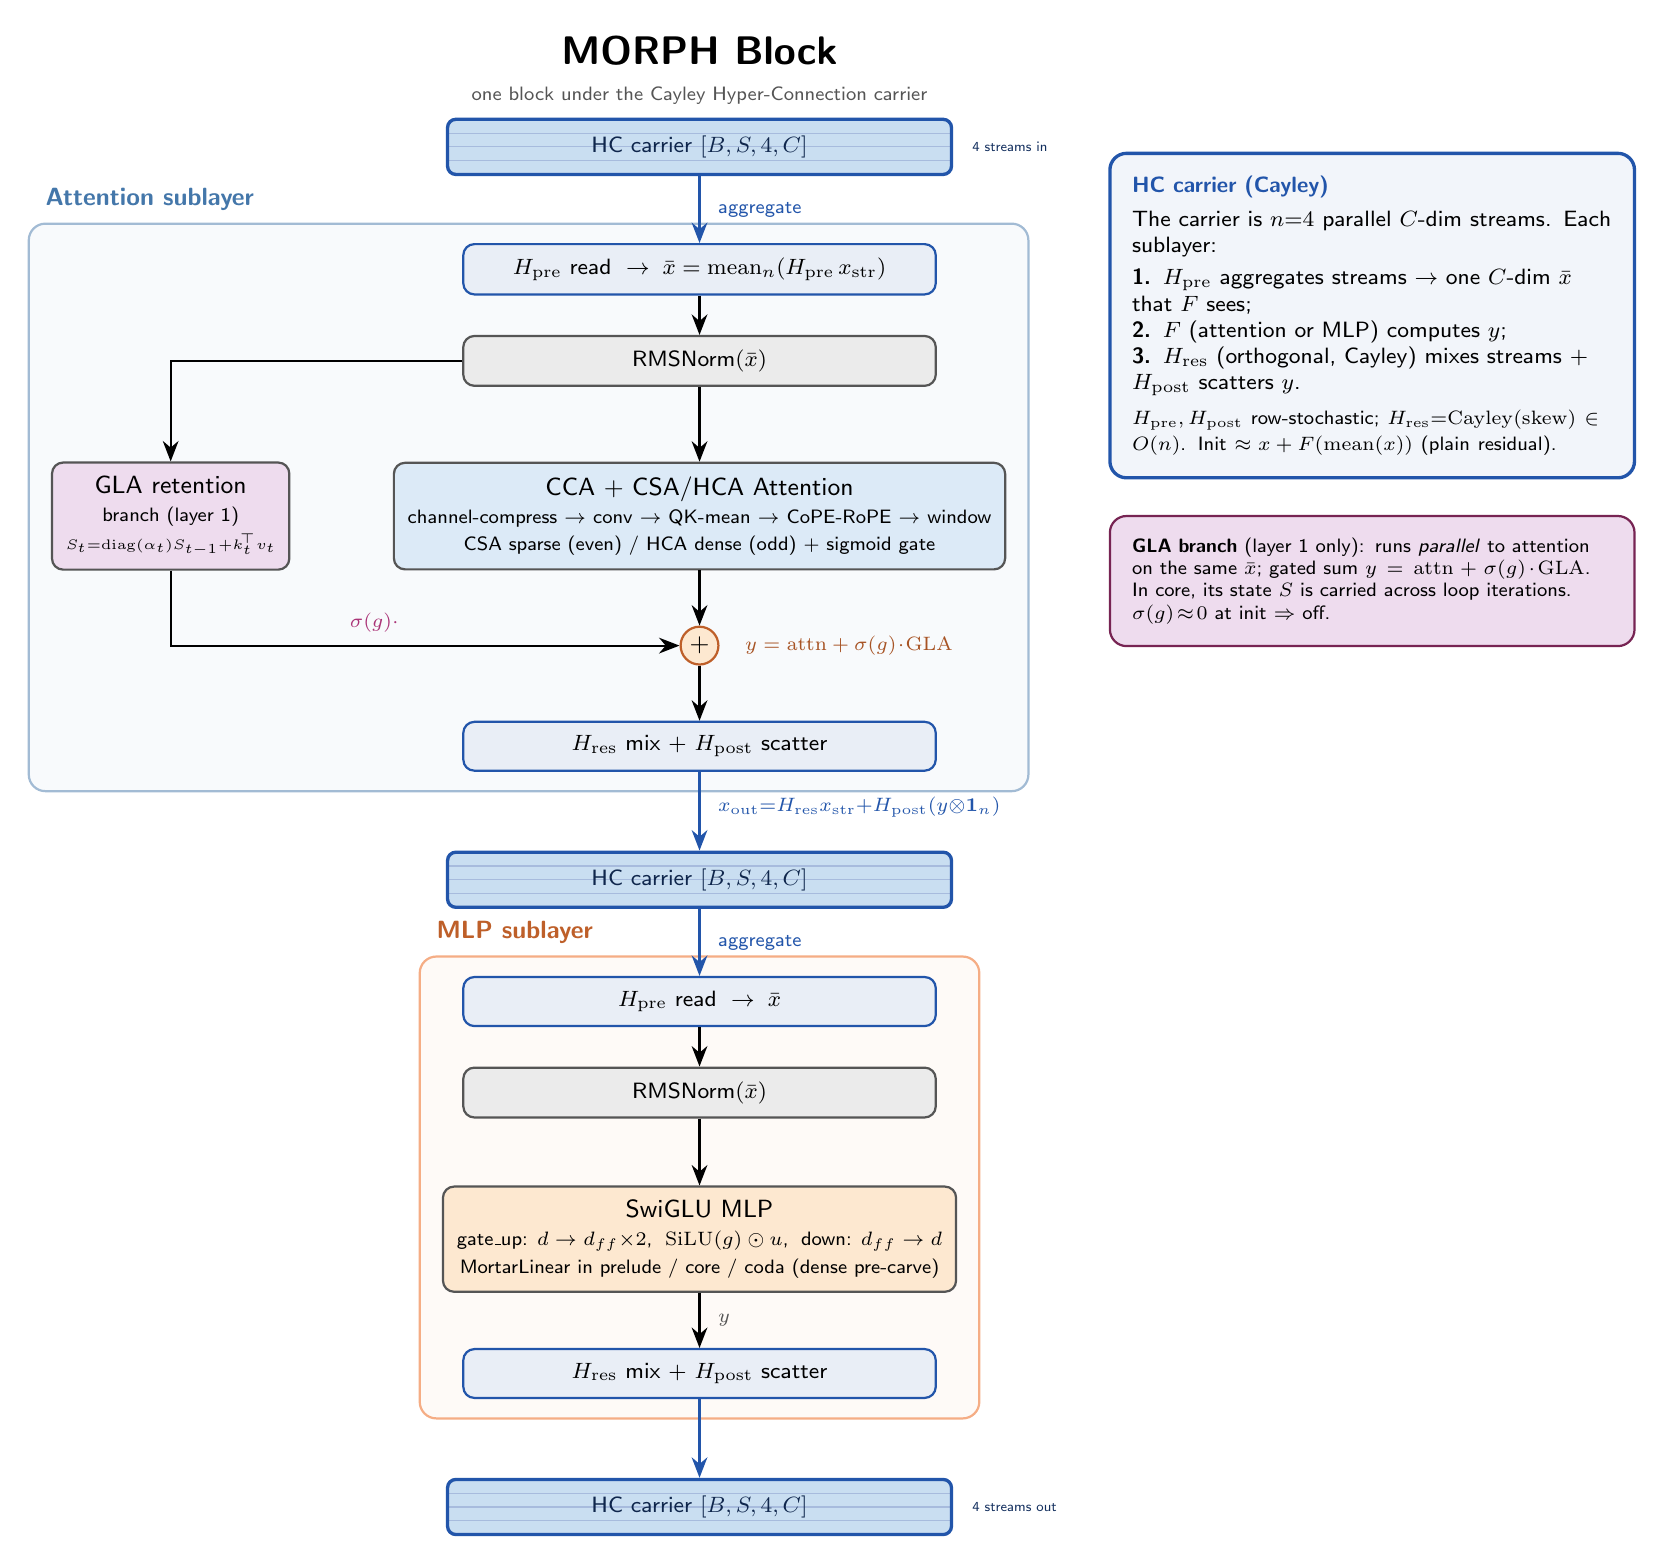
\begin{tikzpicture}[node distance=0.62cm]

% =====================================================================
% MAIN COLUMN (top -> bottom)
% =====================================================================
\node[carrierbar] (cin) {HC carrier $[B,S,4,C]$};
\node[tiny, text=hcC!55!black, anchor=west] at ($(cin.east)+(0.12,0)$) {4 streams in};

% ── ATTENTION SUBLAYER ───────────────────────────────────────────────
\node[Bs, fill=hcC!10, draw=hcC, below=0.85cm of cin] (preA) {
  $H_{\mathrm{pre}}$ read \;$\to\;\bar{x}=\mathrm{mean}_n(H_{\mathrm{pre}}\,x_{\mathrm{str}})$};
\draw[A, hcC] (cin) -- (preA) node[midway, right=3pt, sub, text=hcC]{aggregate};

\node[Bs, fill=fGray, below=0.5cm of preA] (normA) {RMSNorm$(\bar{x})$};
\draw[A] (preA) -- (normA);

\node[B, fill=fBlue, below=0.95cm of normA, minimum height=1.3cm] (attn) {
  CCA + CSA/HCA Attention\\[-1pt]
  {\scriptsize channel-compress $\to$ conv $\to$ QK-mean $\to$ CoPE-RoPE $\to$ window}\\[-1pt]
  {\scriptsize CSA sparse (even) / HCA dense (odd) + sigmoid gate}};
\draw[A] (normA) -- (attn);

% GLA parallel branch (layer 1)
\node[B, fill=fPurple, left=1.3cm of attn, minimum width=2.7cm, minimum height=1.3cm] (gla) {
  GLA retention\\[-1pt]{\scriptsize branch (layer 1)}\\[-1pt]
  {\tiny $S_t{=}\mathrm{diag}(\alpha_t)S_{t-1}{+}k_t^{\!\top}v_t$}};
\draw[A] (normA.west) -| (gla.north);

\node[draw=cbOrange!80!black, thick, circle, fill=fOrange, inner sep=1.5pt,
      below=0.7cm of attn, font=\small] (yA) {$+$};
\draw[A] (attn) -- (yA);
\draw[A] (gla.south) |- (yA) node[pos=0.7, above=1pt, sub, text=cbPurple]{$\sigma(g)\cdot$};
\node[sub, text=cbOrange!70!black, right=0.2cm of yA]
  {$y=\mathrm{attn}+\sigma(g)\!\cdot\!\mathrm{GLA}$};

\node[Bs, fill=hcC!10, draw=hcC, below=0.7cm of yA] (postA) {
  $H_{\mathrm{res}}$ mix $+$ $H_{\mathrm{post}}$ scatter};
\draw[A] (yA) -- (postA);

% attention group box (drawn BEFORE the carrier so the carrier stays outside it)
\begin{scope}[on background layer]
  \node[draw=cbBlue!50, thick, rounded corners=6pt, fill=cbBlue!4,
        fit=(preA)(normA)(attn)(gla)(yA)(postA), inner xsep=8pt, inner ysep=7pt] (AG) {};
\end{scope}
% ── MID CARRIER ──────────────────────────────────────────────────────
\node[carrierbar, below=1.0cm of postA] (cmid) {HC carrier $[B,S,4,C]$};
\draw[A, hcC] (postA) -- (cmid.north)
  node[pos=0.45, right=3pt, sub, text=hcC]
  {$x_{\mathrm{out}}{=}H_{\mathrm{res}}x_{\mathrm{str}}{+}H_{\mathrm{post}}(y{\otimes}\mathbf{1}_n)$};

% ── MLP SUBLAYER ─────────────────────────────────────────────────────
\node[Bs, fill=hcC!10, draw=hcC, below=0.85cm of cmid] (preM) {
  $H_{\mathrm{pre}}$ read \;$\to\;\bar{x}$};
\draw[A, hcC] (cmid) -- (preM) node[midway, right=3pt, sub, text=hcC]{aggregate};
\node[Bs, fill=fGray, below=0.5cm of preM] (normM) {RMSNorm$(\bar{x})$};
\draw[A] (preM) -- (normM);
\node[B, fill=fOrange, below=0.85cm of normM, minimum height=1.15cm] (mlp) {
  SwiGLU MLP\\[-1pt]
  {\scriptsize gate\_up: $d\to d_{ff}{\times}2$,\; $\mathrm{SiLU}(g)\odot u$,\; down: $d_{ff}\to d$}\\[-1pt]
  {\scriptsize MortarLinear in prelude / core / coda (dense pre-carve)}};
\draw[A] (normM) -- (mlp);
\node[Bs, fill=hcC!10, draw=hcC, below=0.7cm of mlp] (postM) {
  $H_{\mathrm{res}}$ mix $+$ $H_{\mathrm{post}}$ scatter};
\draw[A] (mlp) -- (postM) node[midway, right=3pt, sub, text=bdr]{$y$};

\begin{scope}[on background layer]
  \node[draw=cbOrange!60, thick, rounded corners=6pt, fill=cbOrange!4,
        fit=(preM)(normM)(mlp)(postM), inner xsep=8pt, inner ysep=7pt] (MG) {};
\end{scope}
% ── OUT CARRIER ──────────────────────────────────────────────────────
\node[carrierbar, below=1.0cm of postM] (cout) {HC carrier $[B,S,4,C]$};
\draw[A, hcC] (postM) -- (cout.north);
\node[tiny, text=hcC!55!black, anchor=west] at ($(cout.east)+(0.12,0)$) {4 streams out};

% ── Title ────────────────────────────────────────────────────────────
\node[font=\Large\sffamily\bfseries, above=0.55cm of cin] (title) {MORPH Block};
\node[sub, text=bdr, below=0.04cm of title]
  {one block under the Cayley Hyper-Connection carrier};

% =====================================================================
% RIGHT: explainer + alternatives
% =====================================================================
\node[draw=hcC, very thick, rounded corners=6pt, fill=hcC!6,
      anchor=north west, text width=6.1cm, inner sep=8pt,
      font=\footnotesize\sffamily, align=left] at ($(AG.north east)+(1.0,0.9)$) (key) {%
  \textbf{\textcolor{hcC}{HC carrier (Cayley)}}\\[3pt]
  The carrier is $n{=}4$ parallel $C$-dim streams. Each sublayer:\\[2pt]
  \textbf{1.} $H_{\mathrm{pre}}$ aggregates streams $\to$ one $C$-dim $\bar{x}$ that $F$ sees;\\
  \textbf{2.} $F$ (attention or MLP) computes $y$;\\
  \textbf{3.} $H_{\mathrm{res}}$ (orthogonal, Cayley) mixes streams $+$ $H_{\mathrm{post}}$ scatters $y$.\\[3pt]
  {\scriptsize $H_{\mathrm{pre}},H_{\mathrm{post}}$ row-stochastic; $H_{\mathrm{res}}{=}\mathrm{Cayley}(\mathrm{skew})\in O(n)$.
  Init $\approx x+F(\mathrm{mean}(x))$ (plain residual).}};

\node[draw=cbPurple!70!black, thick, rounded corners=6pt, fill=fPurple,
      anchor=north west, text width=6.1cm, inner sep=8pt,
      font=\scriptsize\sffamily, align=left, below=0.45cm of key] (glan) {%
  \textbf{GLA branch} (layer 1 only): runs \emph{parallel} to attention on the same
  $\bar{x}$; gated sum $y=\mathrm{attn}+\sigma(g)\!\cdot\!\mathrm{GLA}$. In core, its state
  $S$ is carried across loop iterations. $\sigma(g)\!\approx\!0$ at init $\Rightarrow$ off.};

% Sublayer labels (drawn last; south-west anchor + small lift clears the border)
\node[font=\small\sffamily\bfseries, text=cbBlue, anchor=south west,
      fill=white, inner sep=2pt]
  at ([xshift=0.15cm, yshift=0.08cm] AG.north west) {Attention sublayer};
\node[font=\small\sffamily\bfseries, text=cbOrange!80!black, anchor=south west,
      fill=white, inner sep=2pt]
  at ([xshift=0.15cm, yshift=0.08cm] MG.north west) {MLP sublayer};

\end{tikzpicture}
\end{document}
